\documentclass[10pt, compress]{beamer}

% \usetheme{m}

\usepackage{booktabs}
\usepackage[scale=2]{ccicons}
\usepackage{minted}
          
\usepackage{tikz}
\usemintedstyle{trac}

\title{Joint Causal Inference (JCI) and protein signalling networks}
\subtitle{Applying the JCI framework to real-world data}
\date{\today}
\author{Alex Khawalid\\\textbf{Supervisor:} Sara Magliacane}
\institute{Universiteit van Amsterdam}

\begin{document}

\maketitle

\begin{frame}
    \frametitle{Introduction}
    The following topics will be discussed
    \begin{itemize}
        \item What is JCI?
        \item What will be researched in this thesis?
        \item What method will be used?
        \item What kind of schedule can be expected?
    \end{itemize}
\end{frame}

\begin{frame}
    \frametitle{What is JCI?}
    \textbf{Preliminary knowledge to understand the problem}
    \begin{itemize}
        \item \textit{Causal Discovery:} \begin{itemize}
            \item a field in statistics
            \item aims to uncover causal relations
        \end{itemize}
        \item \textit{Causal relations:}\begin{itemize}
            \item given an intervention that changes X, if Y changes then X causes Y
            \item can be represented by causal graphs
        \end{itemize}
        \item \textit{JCI:} \begin{itemize}
            \item a framework to do causal discovery
            \item currently implemented with Ancestral Causal Inference with Determinism (ACID)
        \end{itemize}
        \item \textit{ACID:} \begin{itemize}
            \item a method for causal discovery
            \item produces ancestral structure instead of causal DAG
            \item can deal with latent variables
        \end{itemize}
    \end{itemize}
\end{frame}

\begin{frame}{What is JCI?} 
    % explain difference DAG vs Causal DAG vs Ancestral Structure
    % explain what edge JCI has over other methods
    % explain ancestral structure vs causal DAG
    % explain less experimental data necessary
    % multiple datasets
    
  \begin{figure}
    \centering
    \includegraphics[width=\textwidth]{assignment4_cmap.png}
    \caption{An overview of how JCI fits into the bigger picture}
  \end{figure}
\end{frame}

\section{Research question}
\begin{frame}
    \frametitle{Research question}
    \begin{itemize}
        \item \textbf{Main goal of thesis:}
            \begin{itemize}[<+- | alert@+>]
                \item How does JCI perform on a real-world dataset? 
            \end{itemize}
    
        \item\textbf{The problem:}
            \begin{itemize}[<+- | alert@+>]
                \item JCI cannot use the required number of variables
            \end{itemize}
    
        \item\textbf{Solution:}
            \begin{itemize}[<+- | alert@+>]
                \item Scale JCI to enable the use of more variables
            \end{itemize}
    \end{itemize}
\end{frame}


\section{Approach}
\begin{frame}
    \frametitle{Approach}
    \textbf{How can JCI be scaled to a larger number of variables?}
    
    \textbf{Proposed method:}
    \begin{itemize}
        \item Assign subsets of variables within data
        \item Combine causal graphs from JCI
        \item Not trivial
        \item Evaluate with Recall, Precision and running time
        % approximation of unnormalized probability of edges
        % logical that i dont know
    \end{itemize}
    
    \tikzstyle{var}=[circle,draw=black,fill=white,thin,minimum size=18pt,inner sep=0pt]
    \tikzstyle{arr}=[->,>=stealth,draw=black,thick]
    \begin{tikzpicture}
        \node[var] (X1) at (-1,0) {X};    
        \node[var] (X2) at (1,0) {Y};
    	\node[var] (X3) at (0, 1) {Z};
    	\draw[arr] (X1) -- (X2) node [midway, above, draw=none, fill=none] {\scriptsize{10}};
        \draw[arr] (X3) -- (X2) node [midway, above, draw=none, fill=none] {\scriptsize{130}};
        \draw[arr] (X3) -- (X1) node [midway, above, draw=none, fill=none] {\scriptsize{50}};
    \end{tikzpicture}
     
    \begin{tikzpicture}
        \node[var] (X1) at (-1,0) {X};    
        \node[var] (X2) at (1,0) {A};
    	\node[var] (X3) at (0, 1) {B};
    	\draw[arr] (X1) -- (X2) node [midway, above, draw=none, fill=none] {\scriptsize{300}};
        \draw[arr] (X3) -- (X2) node [midway, above, draw=none, fill=none] {\scriptsize{150}};
        \draw[arr] (X3) -- (X1) node [midway, above, draw=none, fill=none] {\scriptsize{100}};
     \end{tikzpicture}
\end{frame}

\section{Schedule}
\begin{frame}
    \frametitle{Schedule}
    \textbf{Milestones}
    \begin{itemize}
        \item Understand codebase and get it working
        \item Efficient subset assignment
        \item Find theoretically sound graph combination method
        \item Apply and compare methods
    \end{itemize}
    
\end{frame}

\begin{frame}
    \frametitle{Schedule}
    \begin{figure}
        \centering
        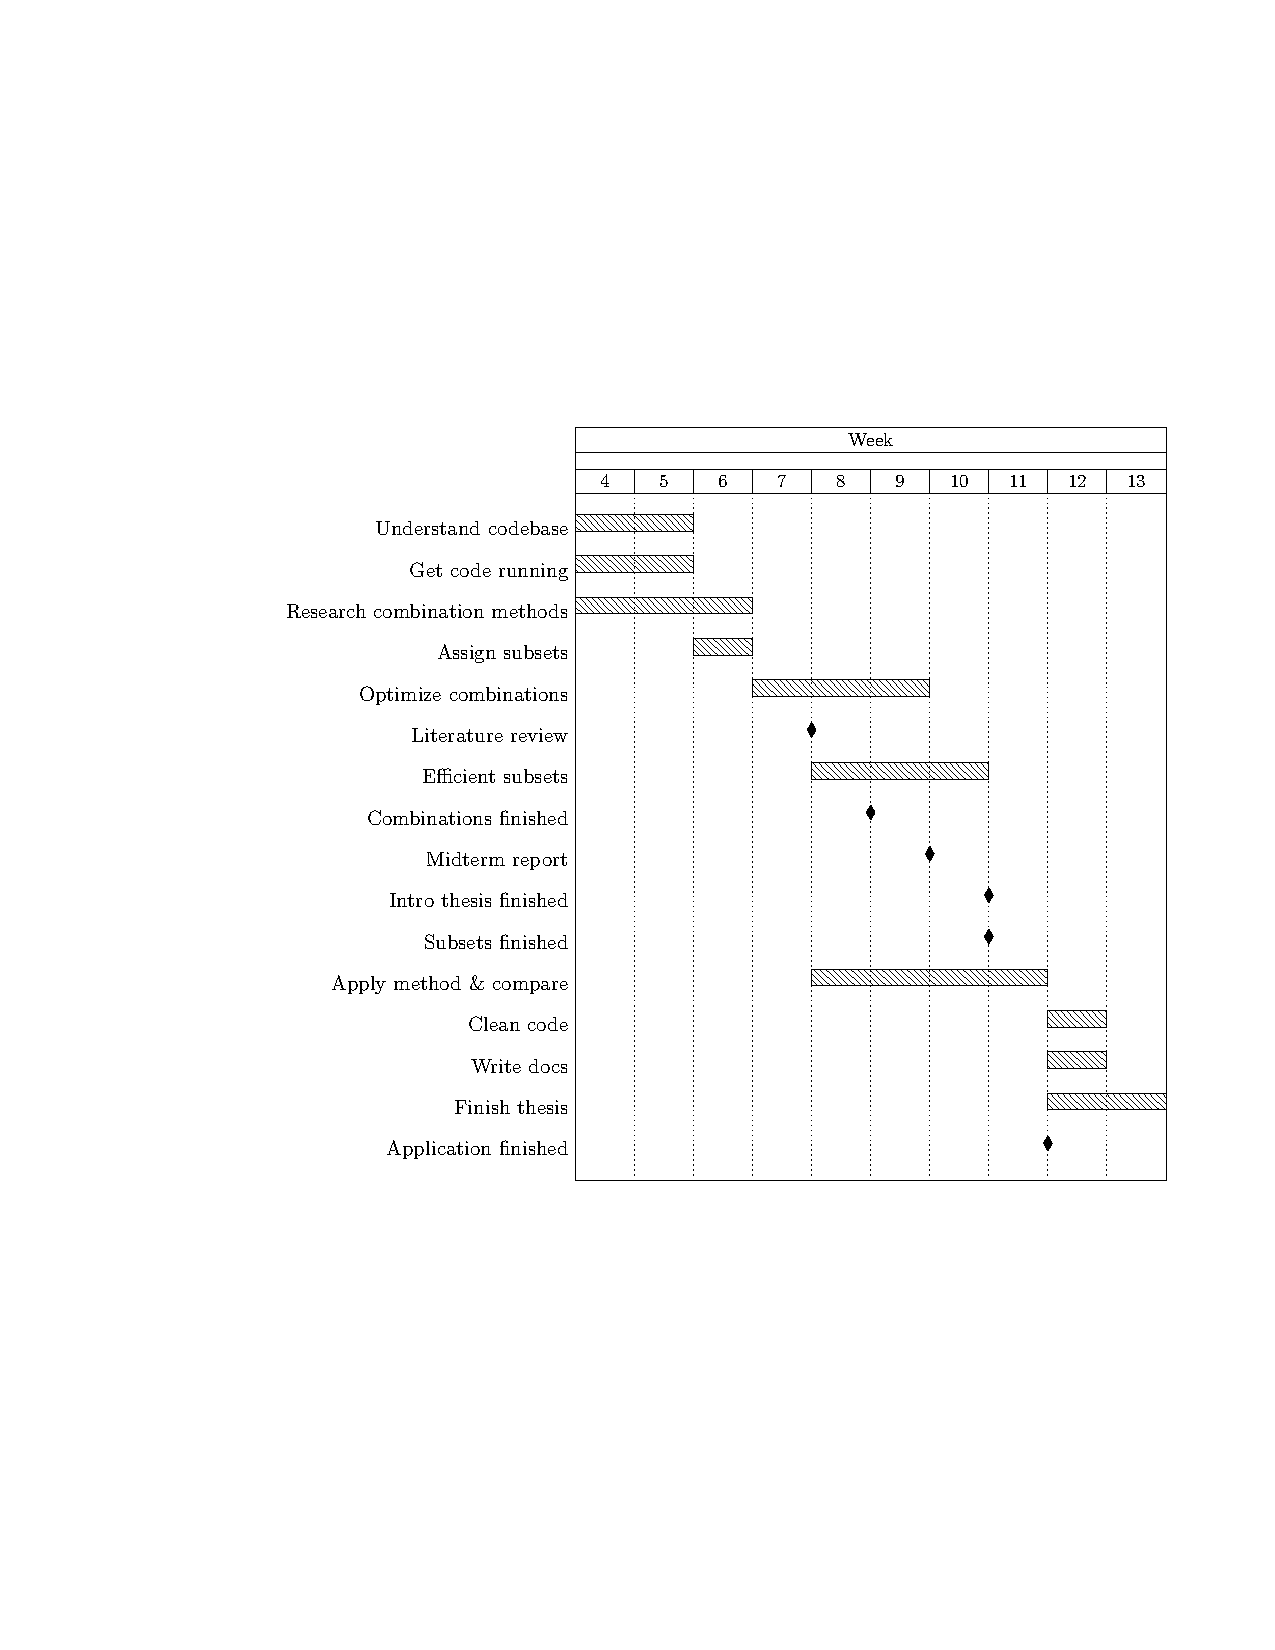
\includegraphics[width=\textwidth]{ScriptieOpdrachten.pdf}
        \caption{Caption}
        \label{fig:my_label}
    \end{figure}
\end{frame}

\plain{}{Questions?}

\end{document}
